Please describe the achieved outcomes of the project.
If possible, please provide figures showing the described outcomes.
Please confront them with the objectives of the project.
This part should be between 2000 and 10,000 characters long.
Please use Times New Roman font, 12 pts, 1.5 spacing.
Full description of solutions that were worked out and project outcomes, if any, should be presented in annexes.
\begin{figure}[H]
    \centering
    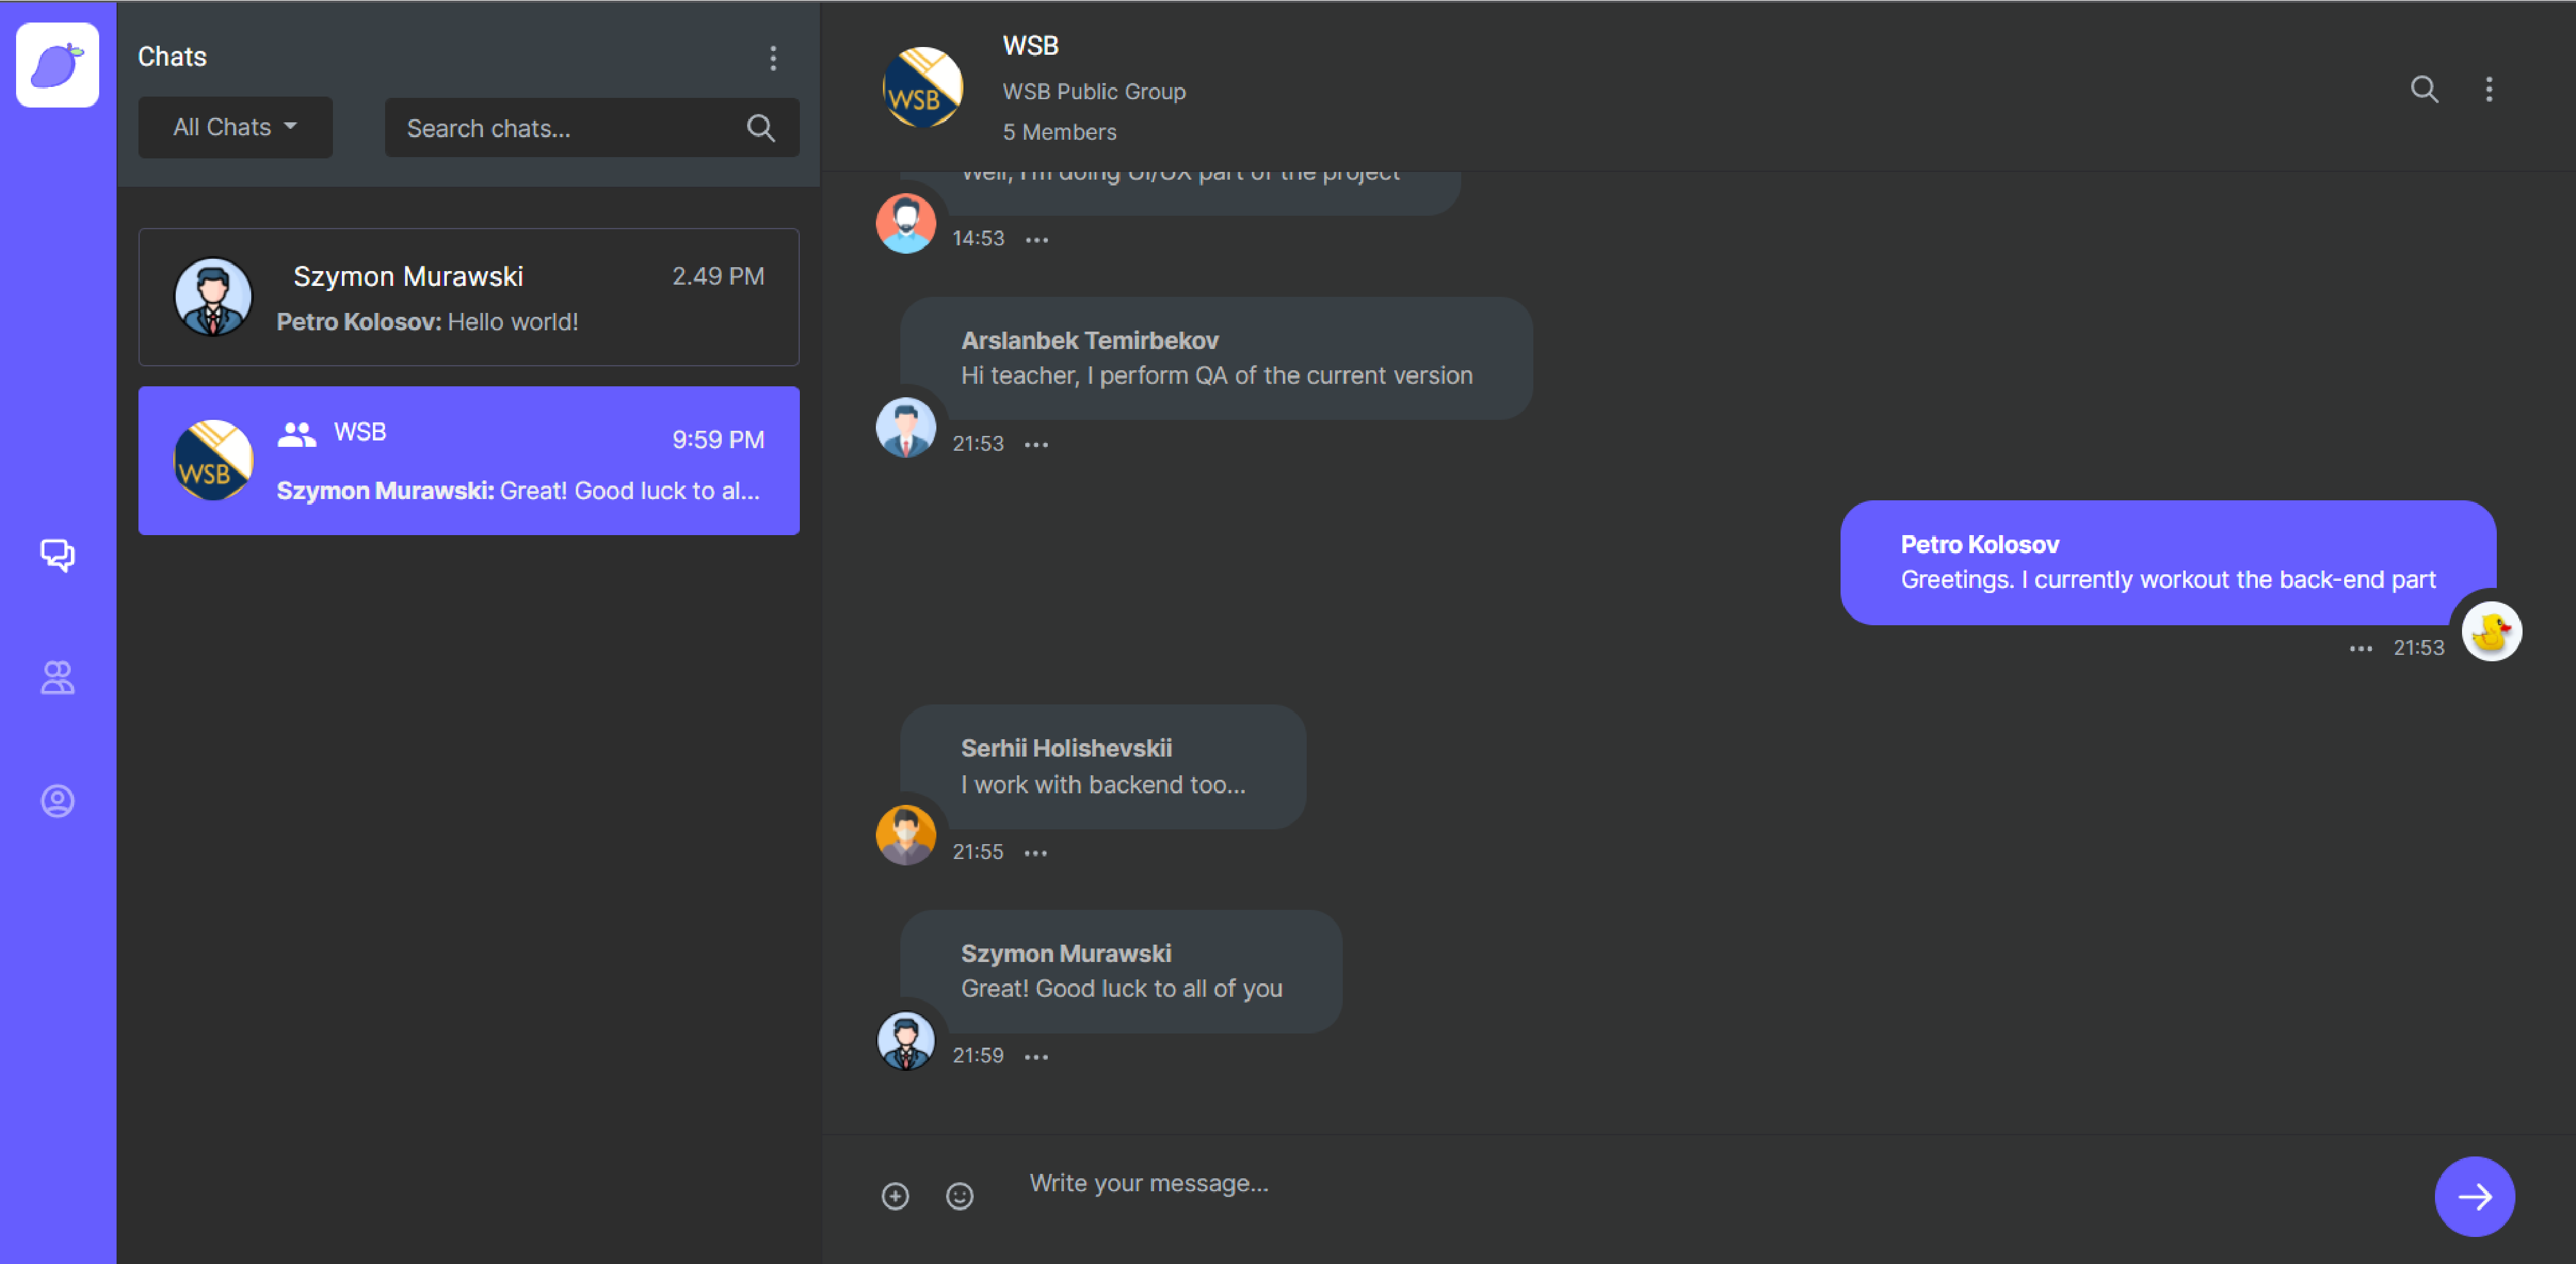
\includegraphics[width=1\textwidth]{Pictures/Messenger-1}
    \caption{Secret chat encryption concept diagram. Source: }\label{fig:figure5}
\end{figure}

\begin{enumerate}
    \item Element responsible for getting user's chats list so that functional requirement "As an authorized user,
    I want to view a message history of particular chat or group so that I see a list of my active chats on the UI" is satisfied.
    \item Element responsible for searching chats by display name and displaying it so that functional requirments
    "As an authorized user, I want to search public groups by title so that I enter display name to specified field,
    click button "Search chats" and see results." and "As a registered user, I want to join public groups so that I click button "Join group"
    to join the group." is satisfied.
    \item Element responsible for creating groups so that functional requirment "As a registered user, I want to tap "Create channel"
    so that I create a new channel of the one of the types: Private channel, Public channel, Readonly channel".
    \item Element resonsible for filtring chats so that functional requirement "As an authorized user,
    I want to filter a message history of particular chat or group so that I see a filtered list of my active chats on the UI." is satisfied.
    \item Element responsible for archiving and leaving from the particular chat, so that functional requirements "As registered user, I want to tap
    "Leave" so that I leave from specified chat or channel.", "As a registered user, I want to tap "Archive" so that I archive the specified chat
    or channel.", "As a registered user, I want to tap "Un-archive" so that I un-archive the specified
    archived chat or channel." is satisfied.
    \item Element responsible for entering the text and sending a message by enter, so that functional requirement "As an authorized user,
    I want to send a text message so that other members of the group see the message I sent." is satisfied.
    \item Element responsible for adding emoji to message, so that functional requirement "As an authorized user, I want to add an emoji
    to the message so that other members of the group see the message with emoji I sent." is satisfied.
    \item Element responsible for adding attachments to the message, so that functional requirement "As an authorized user,
    I want to add an attachment to the message so that other members of the group see the message with attachment I sent." is satisfied.
    \item Element responsible for replying to message, so that functional requirement "As registered user,
    I want tap "Reply" so that I want reply to the particular message" is satisfied.
    \item Element responsible for editing and deleting a message so that functional requirements "As an authorized user, I want to tap
    "Edit" on my message so that other members of the group see the message I edited.", "As an authorized user, I want to tap "Delete"
    on my message so that my message is deleted for all members of the group." is satisfied.
    \item Element responsible for sending message if message text field is not empty so that functional requirement "
    \item Element responsible for seraching messages in the particular chat so that functional requirement "As an authorized user, I want to search messages
    in particular chat so that I see the results in messages window of the chat." is satisfied.
    \item Element responsible for navigation about main page, contacts page and personal information page so that functional requirement
    "As an authorized user, I want navigation about pages so that I can navigate to the contacts and personal information page from main page and vice versa."
    is satisfied.
\end{enumerate}

\begin{figure}[H]
    \centering
    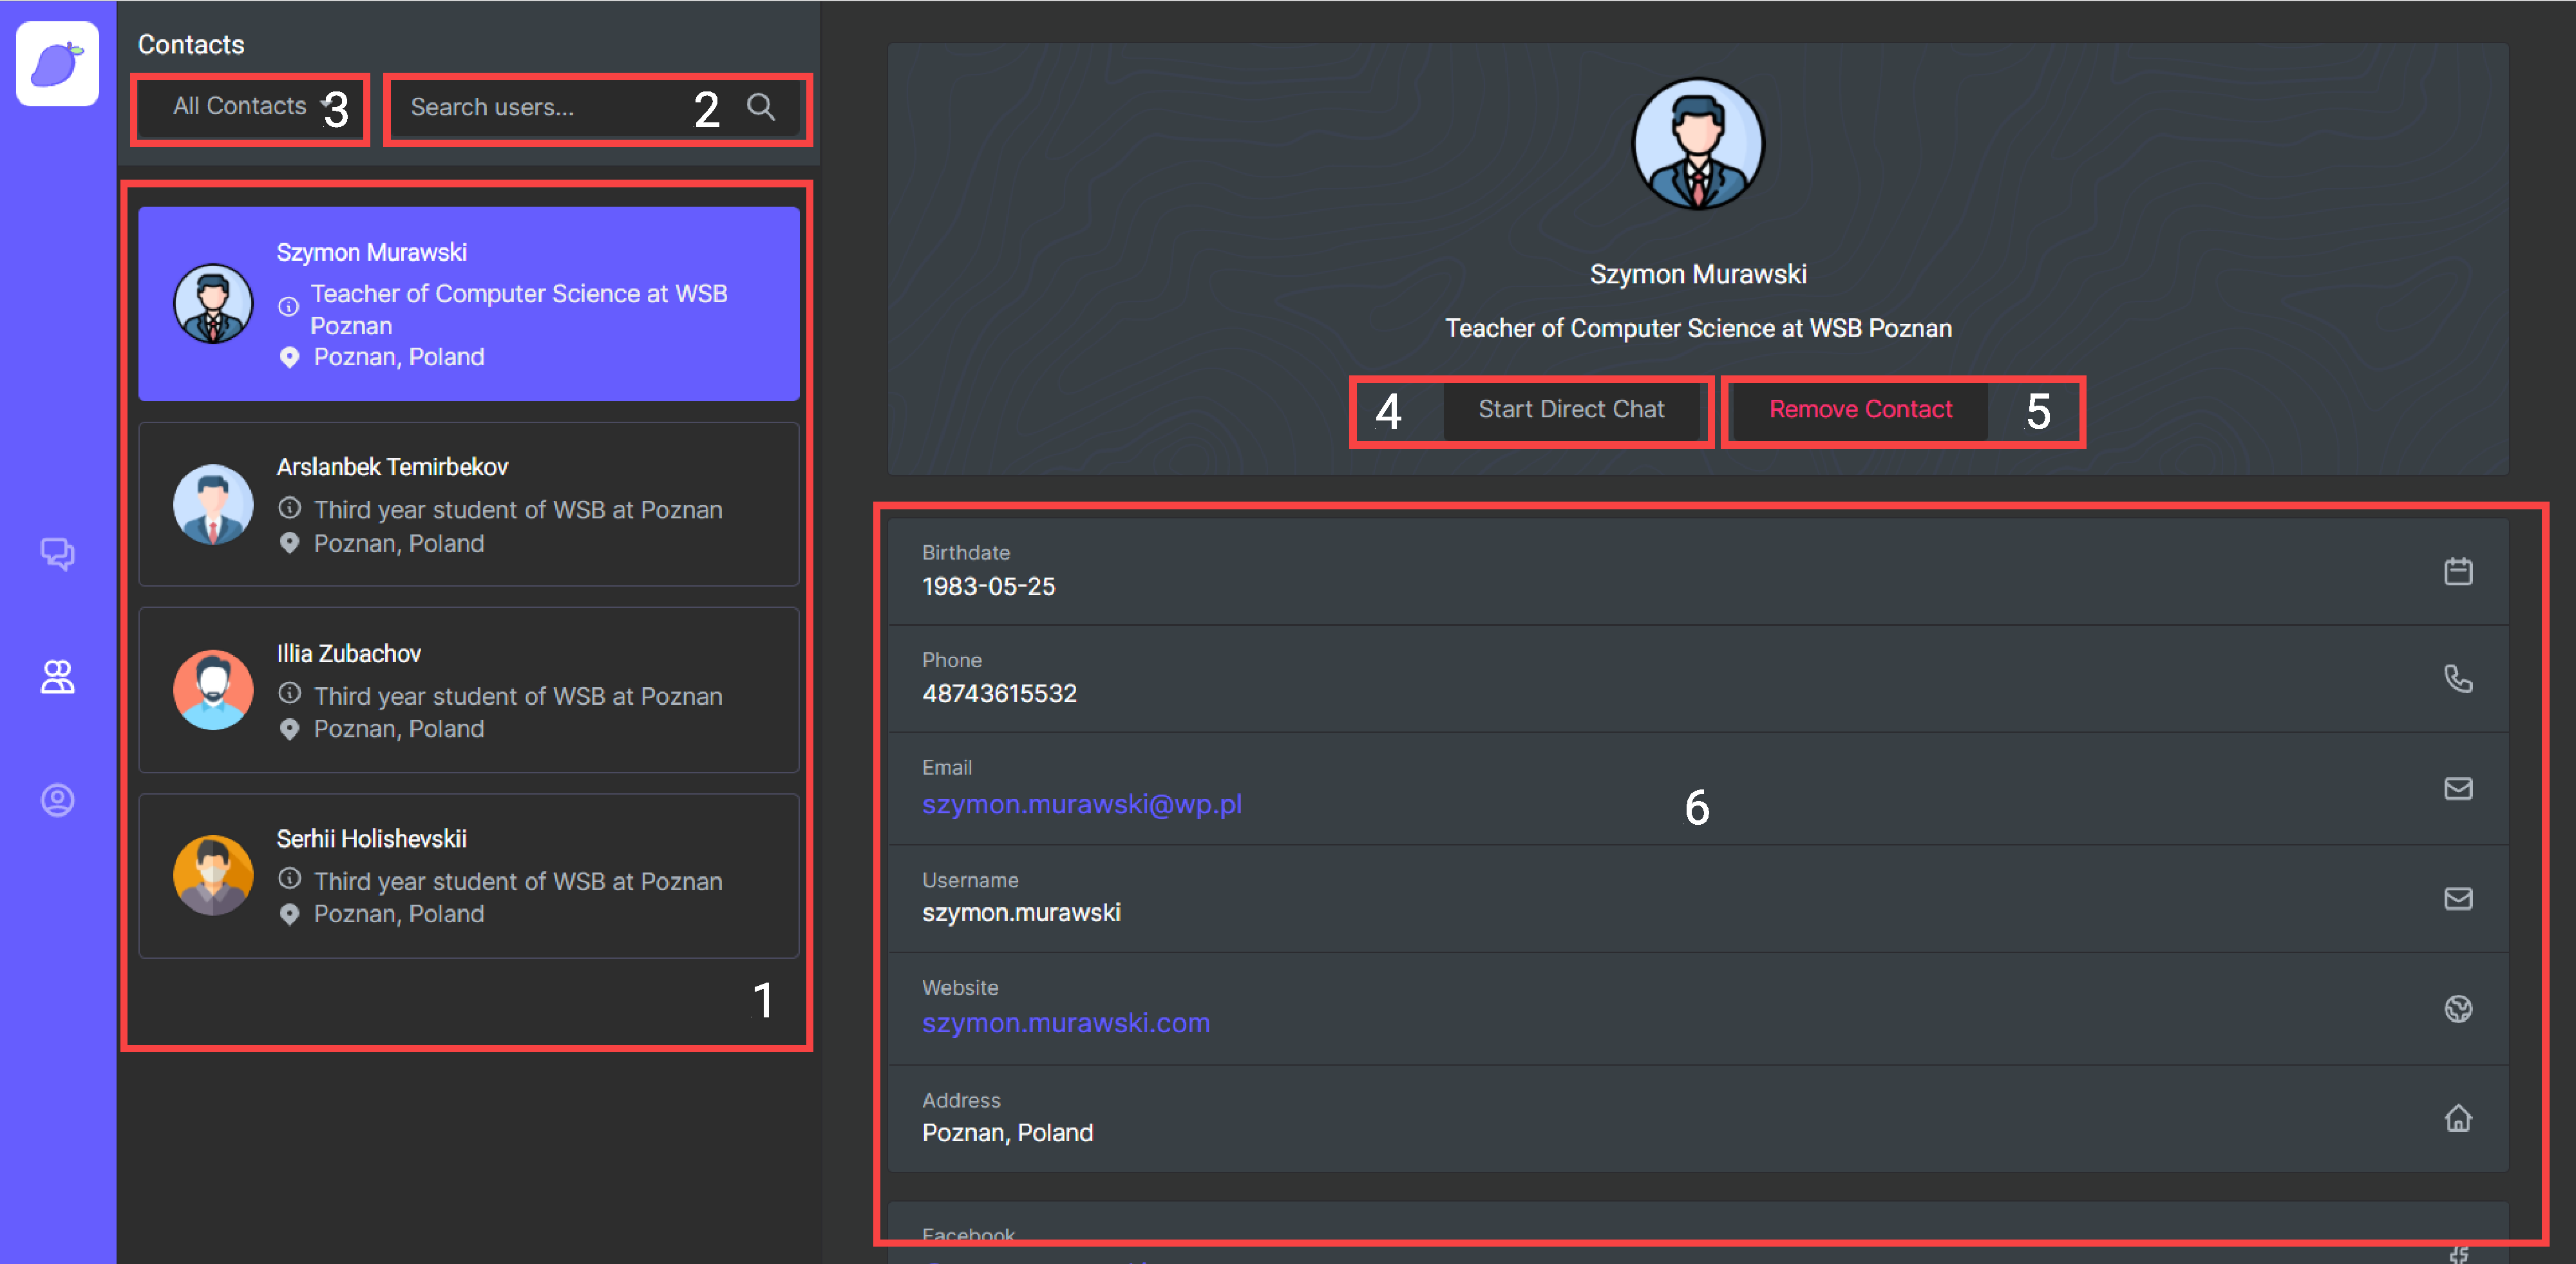
\includegraphics[width=1\textwidth]{Pictures/Messenger-2}
    \caption{Secret chat encryption concept diagram. Source: }\label{fig:figure10}
\end{figure}
\begin{enumerate}
    \item Element responsible for output user's contacts so that functional requirement "As an authorized user, I want to see my contact list so that there
    is a list of users who are my contacts." is satisfied.
    \item Element responsible for searching users so that functional requirement "As an authorized user, I want to search users so that
    I write user display name or phone number of e-mail address to specified input, click "Search user" button and see results" is stasfied.
    \item Element responsible for filtering contacts so that functional requirement "As an authorized user, I want to search users so that I write
    user display name or phone number of e-mail address to specified input, click "Search user" button and see results" is satisfied.
    \item There is a button, clicking on which you can start chat with a specific user.
    \item Element responsible for creating chat with specified user so that functional requirement "As an authorized user, I want to tap "Start chat" so that
    create chat with specified user/contact" is satisfied.
    \item Element responsible for deleting user form contacts so that functional requirement "As an authorized user, I want to remove the user from my
    contact list so that I click "Remove contact" button on user profile and remove him from my contact list." is satisfied.
    \item Element responsible for the output specified user's info so that functional requirement "As an authorized user, I want to tap on specified contact
    so that I want see user's information." is satisfied.
\end{enumerate}

\begin{figure}[H]
    \centering
    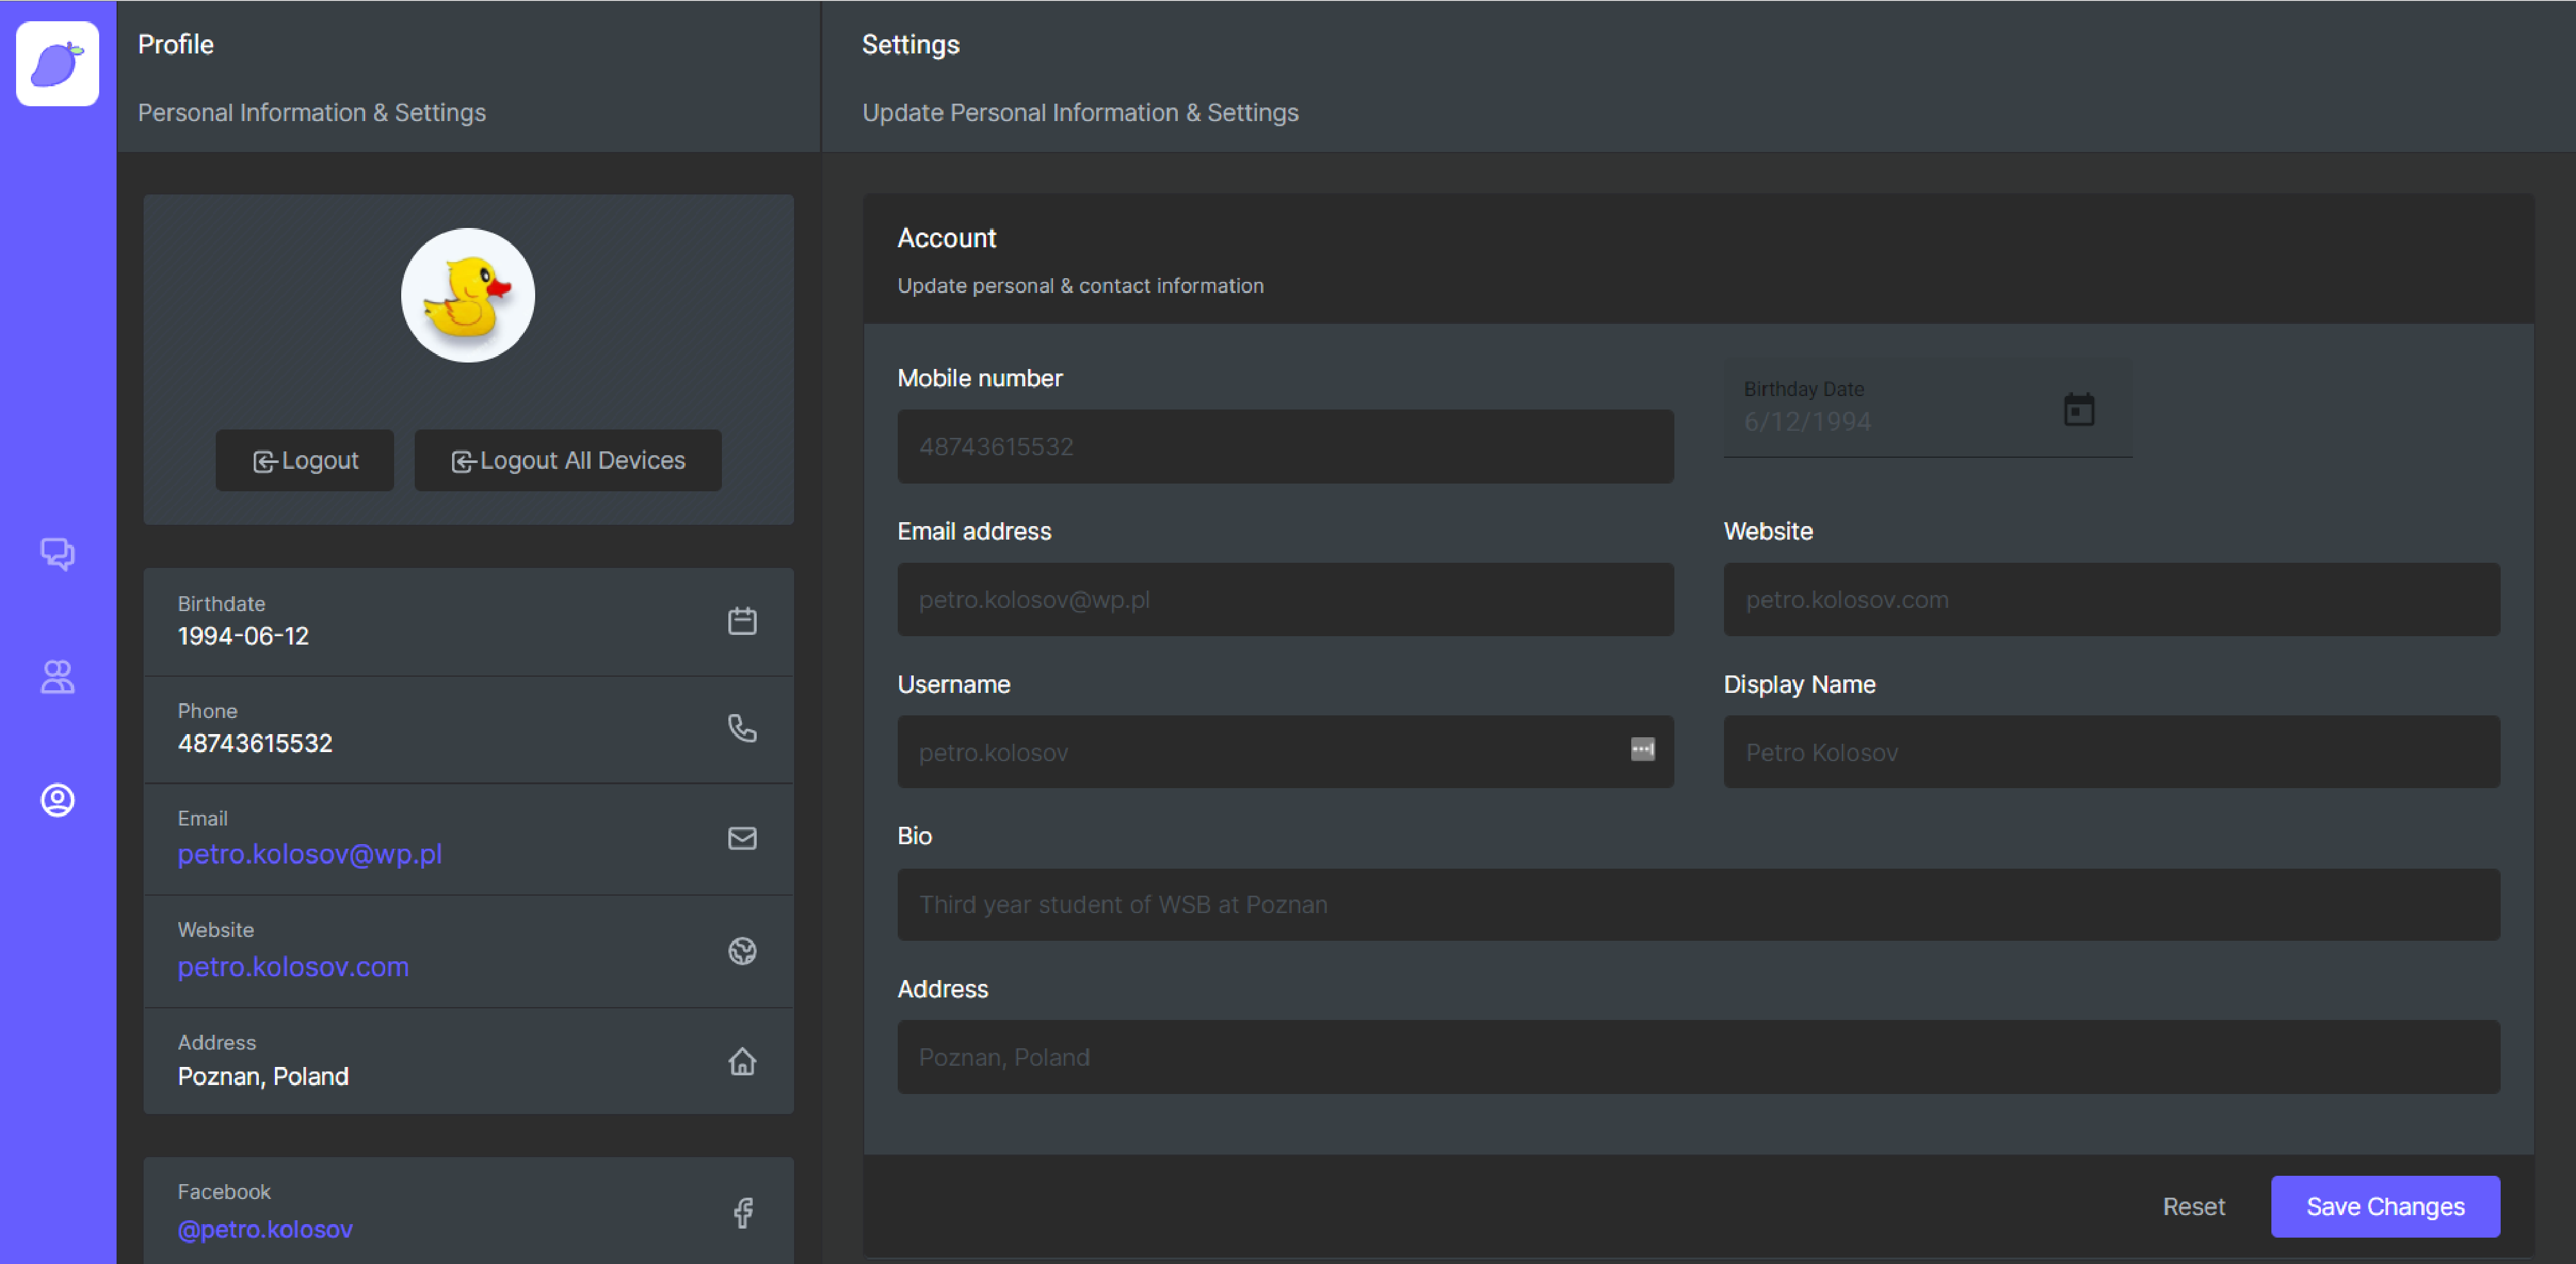
\includegraphics[width=1\textwidth]{Pictures/Messenger-3}
    \caption{Secret chat encryption concept diagram. Source: }\label{fig:figure11}
\end{figure}
\begin{enumerate}
    \item Element responsible for log out from specified device so that functional requirement "As an authorized user, I want to tap
    "Logout" button so that current device will be logged out from the system." is satisfied.
    \item Element responsible for log out from all devices so that functional requirement "As an authorized user, I want to tap
    "Logout all" button so that all my authorized devices will be logged out from the system." is satisfied.
    \item Element responsible for output user's avatar so that functional requirement "As an authorized user, I want to navigate to personal information page
    so that I want see my profile picture." is satisfied.
    \item Element responsible for output user's information so that functional requirement
    "As an authorized user, I want to navigate to personal information page so that I want see my personal information." is satisfied.
    \item Element responsible for reset updated personal information so that functional requirement "As an authorized user, I want to
    tap "Reset" so that I want reset my updated(not saved) personal information." is satisfied.
    \item Element responsible for saving personal information so that functional requirement "As an authorized user, I want save my
    updated personal information so that users will see it."
    \item Element responsible for changing personal information so that functional requirement "As an authorized user, I want to
    update my personal information in profile settings so that other users my updated personal information."
\end{enumerate}